%!TEX root = ../template.tex
%%%%%%%%%%%%%%%%%%%%%%%%%%%%%%%%%%%%%%%%%%%%%%%%%%%%%%%%%%%%%%%%%%%%
%% chapter3.tex
%% NOVA thesis document file
%%
%% Chapter with a short laext tutorial and examples
%%%%%%%%%%%%%%%%%%%%%%%%%%%%%%%%%%%%%%%%%%%%%%%%%%%%%%%%%%%%%%%%%%%%
\chapter{Trabalho Realizado}
\label{cha:trabalho_realizado}
O objetivo principal deste tema foi desenvolver um protótipo que seja capaz de construir automaticamente descritores de documentos. Para além de \textit{keywords} explícitas, estes descritores deverão conter \textit{keywords} implícitas que possam estabelecer pontes semânticas entre os documentos. 
A identificação destes elementos implícitos envolve o cálculo de correlações entre pares de expressões relevantes. Considerando que o número destes pares cresce quadraticamente com o número de expressões relevantes do \textit{corpus}, esta computação exige processamento paralelo e distribuído. 
Como foi referido anteriormente, optou-se pelo coeficiente de correlação de Pearson (secção \ref{equa:correlation_Pearson}).

\section{Protótipo - Versão sequencial}

Com vista ao desenvolvimento do protótipo final, é necessária a criação de uma implementação sequencial da fórmula de correlação de Pearson. Versão sequencial esta que para além de nos ajudar a decompor a fórmula da correlação de Pearson em sub-funções que podem ser otimizadas, também ajuda a perceber até que ponto e onde é que a fórmula pode ser paralelizável. Para além disso, esta versão sequencial do protótipo vai servir como  base de amostra de correlações entre as várias expressões relevantes, com vista a uma futura comparação de resultados com o protótipo final não puramente sequencial.

A versão sequencial já foi construída com recurso à linguagem de programação Java. Optou-se por esta linguagem porque oferece uma quantidade considerável de bibliotecas úteis para ler documentos de texto e extrair/comprimir documentos no decorrer da execução do programa. O ambiente de teste tanto desta versão como do protótipo final é um \textit{corpus} extraído do Wikipédia que contém 23218 documentos de texto (todos eles comprimidos em modo \textit{.zip}), perfazendo um total de aproximadamente 50 milhões de palavras. Para que existam ERs para correlacionar, estas têm de ser extraídas a partir do \textit{corpus}. Extração esta que é feita utilizando o algoritmo \textit{LocalMaxs}, como referido acima (final de secção \ref{sec:extractores}). 

\subsection{Decomposição da correlação de Pearson}
Após a obtenção das ERs, o passo que se seguiu foi decompor a fórmula do coeficiente de correlação de Pearson em sub-funções apresentada na secção \ref{equa:correlation_Pearson}. Esta fórmula tem como numerador a covariância entre duas ERs ($E_{1} e E_{2}$), e como denominador sobre o produto entre as raízes quadradas das covariâncias de cada ER com elas próprias. Achamos por bem começar por decompor a função $cov(E_{1}, E_{2})$. O resultado da decomposição está descrito abaixo:
%\begin{equation}
%\begin{aligned}
%    cov(E_{1}, E_{2}) = & [ \sum_{d \epsilon \#Docs} (f_{r}(E_{1}, d)\cdot f_{r}(E_{2}, d)) \\                          & -(f_{r}(E_{2},\cdot) \cdot \!\!\sum_{d \epsilon \#Docs} f_{r}(E_{1},d)) \quad - (f_{r}(E_{1}, \cdot) \cdot \!\!\sum_{d \epsilon \#Docs} f_{r}(E_{2}, d))  \\
%                        & +(\sum_{d \epsilon \#Docs} f_{r}(E_{1}, \cdot) \cdot f_{r}(E_{2},\cdot)) ]
%\end{aligned}
%\end{equation}%
\begin{equation}
\begin{aligned}
    cov(E_{1}, E_{2}) = & [ A  & -B & + C ]
\end{aligned}
\end{equation}

Podemos observar que nesta expressão falta o primeiro fator relativamente à fórmula (equação \ref{covarianceXY}) (o inverso do número total de documentos menos um), pois este fator anula-se na fórmula da correlação (equação \ref{equa:correlation_Pearson}). Assim, não é necessário incluir este fator. Podemos identificar três parcelas distintas para a implementação desta expressão:
\begin{description}
\item[A:] Soma do produto das frequências relativas de $E_{1} e E_{2}$ no mesmo documento;
\begin{equation}
\begin{aligned}
    \sum_{d \epsilon \#Docs} (f_{r}(E_{1}, d)\cdot f_{r}(E_{2}, d))
\end{aligned}
\end{equation}
\item[B:] subtração entre a soma das frequências relativas de $E_{1}$ nos documentos onde aparece, vezes a frequência média relativa de $E_{2}$, e a soma das frequências relativas de $E_{2}$, vezes a frequência média relativa de $E_{1}$;
\begin{equation}
\begin{aligned}
 (f_{r}(E_{2},\cdot) \cdot \!\!\sum_{d \epsilon \#Docs} f_{r}(E_{1},d)) \quad - (f_{r}(E_{1}, \cdot) \cdot \!\!\sum_{d \epsilon \#Docs} f_{r}(E_{2}, d))
\end{aligned}
\end{equation}
\item[C:] a terceira parcela, a frequência média relativa de $E_{1}$, vezes a frequência média relativa $E_{2}$, vezes o número total de documentos no \textit{corpus}.
\begin{equation}
\begin{aligned}
    \sum_{d \epsilon \#Docs} f_{r}(E_{1}, \cdot) \cdot f_{r}(E_{2},\cdot)
\end{aligned}
\end{equation}
\end{description}

Após a separação da $cov(E_{1} e E_{2})$ em várias parcelas, procedeu-se à decomposição do denominador da fórmula de correlação de Pearson. Decomposição esta que resultou em:
%\begin{equation}
%\begin{aligned}
%\sqrt{cov(E_{i}, E_{i})} = \sqrt{ (\sum_{d \epsilon \#Docs} f_{r}(E_{i}, d)^{2} - (2\times f_{r}(E_{i}, \cdot )^{2} \times \#Docs) + (f_{r}(E_{i}, \cdot )^{2} \times \#Docs) }
%\end{aligned}
%\end{equation}%

\begin{equation}
\begin{aligned}
\sqrt{cov(E_{i}, E_{i})} = \sqrt{ D - E + F }
\end{aligned}
\end{equation}

Analogamente à primeira decomposição, também foi retirado o fator correspondente ao inverso do número total de documentos menos um. Podemos também identificar três parcelas em $\sqrt{cov(E_{i}, E_{i})}$:
\begin{description}
\item[D:] soma do quadrado da frequência relativa de $E_{i}$ em cada documento;
\begin{equation}
\begin{aligned}
\sum_{d \epsilon \#Docs} f_{r}(E_{i}, d)^{2}
\end{aligned}
\end{equation}
\item[E:] multiplica dois pela frequência média relativa de $E_{1}$, vezes o número total de documentos;
\begin{equation}
\begin{aligned}
2\times f_{r}(E_{i}, \cdot )^{2} \times \#Docs
\end{aligned}
\end{equation}
\item[F:] a terceira parcela, representa o produto entre o quadrado da frequência média relativa de $E_{i}$, e o número total de documentos.
\begin{equation}
\begin{aligned}
f_{r}(E_{i}, \cdot )^{2} \times \#Docs
\end{aligned}
\end{equation}
\end{description}

\subsection{Modelo de Programa}
A estrutura deste programa vai ser descrita pela ordem de resolução mais pequena, até à resolução maior. Ou seja, desde a classe que só se responsabiliza por contar o número de ocorrências de uma ER no \textit{corpus}, até à classe principal que controla o fluxo da execução das classes, tal como está exibido na figura \ref{fig:fluxo_execucao_prototipo}. De notar que todos os resultados produzidos pelas classes construídas nesta versão são escritos para ficheiros \textit{.txt}.

Tendo em conta as parcelas que foram decompostas a partir da fórmula de Pearson, podemos concluir que estas dependem maioritariamente do cálculo da frequência relativa de $E_{i}$ num documento (equação \ref{freq_relative}), e da frequência média relativa de $E_{i}$ (equação \ref{freq_rela_average}). Para o cálculo da frequência relativa de $E_{i}$ num documento, foi necessária a criação de duas classes. A classe \textit{ERFile\_Counter}, que conta o número de vezes que uma dada ER aparece num dado documento e \textit{DocsWordCounter} que conta o número total de palavras que um documento contém. A classe construída para calcular a frequência relativa foi \textit{RelativeFreq\_E1InDoc}, que faz uso dos respostas resultantes das duas classes acima descritas. Já no cálculo da frequência média relativa de $E_{i}$, foi criada a classe \textit{AverageRelativeFreq\_E1InAllDocs}, que tal como a classe \textit{RelativeFreq\_E1InDoc}, também faz uso das mesmas classes para efetuar os seus cálculos.

Prossegue-se agora para o nível acima da hierarquia de classes, que é constituída por duas, \textit{CovarianceEi\_Ei} e \textit{CovarianceE1\_E2}. A classe \textit{CovarianceEi\_Ei}, que efetua o cálculo da covariância entre uma ER com ela própria, lê os resultados produzidos pelas classes \textit{RelativeFreq\_E1InDoc} e \textit{AverageRelativeFreq\_E1InAllDocs}. O mesmo acontece para \textit{CovarianceE1\_E2}. 

A partir dos resultados produzidos por \textit{CovarianceEi\_Ei} e \textit{CovarianceE1\_E2}, foi possível implementar a classe \textit{Correlation\_E1\_E2}. Esta tem como objetivo calcular o resultado final do coeficiente de correlação de Pearson.

\begin{figure}[htbp]
	\centering
	\includegraphics[height=1.5in]{LaTeX/Chapters/Figures/FluxoExecucao_VersaoSequencial_Optmized.png}
  \caption{Fluxo de execução da versão sequencial}
  \label{fig:fluxo_execucao_prototipo}
\end{figure}

\subsection{Resultados - Versão Sequencial}
Para além da versão sequencial servir como termo de comparação de resultados, também mostra a necessidade dum ambiente paralelo  e distrubuído (\textit{Hadoop} ou \textit{Spark}) para o cálculo da  correlação de Pearson a um tão grande número de pares de ERs. Os resultados obtidos da correlação entre duas ERs foram entre -1 e 1, como se esperava. Relembrando que, 1 significa fortemente correlacionado e -1 ERs de assuntos tendencialmente "opostos".

Ao longo da construção deste protótipo sequencial, constatou-se que existem precedências entre as várias classes, ou seja, existem as que só podem ser executadas após a execução de outras. Como podemos observar na figura \ref{fig:fluxo_execucao_prototipo}, temos duas classes (\textit{ERFile\_Counter} e \textit{DocsWordCounter}) que dependem diretamente do \textit{corpus}, podendo ser executadas em paralelo, pois não dependem dos resultados uma da outra. Segue-se a execução das  (\textit{RelativeFreq\_E1InDoc} e \textit{AverageRelativeFreq\_E1InAllDocs}), que têm cálculos independentes uma da outra, por isso podem vir a ser executadas em paralelo. No entanto, dependem dos resultados das classes que trabalham diretamente com o \textit{corpus}. De seguida temos as \textit{CovarianceEi\_Ei} e \textit{CovarianceE1\_E2} que dependem dos resultados produzidos pelas classes \textit{RelativeFreq\_E1InDoc} e \textit{AverageRelativeFreq\_E1InAllDocs}. Contudo como executam cálculos independentes um do outro pode ser executadas em paralelo. Por fim temos a classe \textit{CorrelationE1\_E2}, que necessita dos resultados produzidos por \textit{CovarianceEi\_Ei} e \textit{CovarianceE1\_E2}, para poder calcular o resultado final. 


A versão sequencial foi executada num \texit{desktop} com a versão de 64 bits do Windows 10 Pro, um processador Intel Core i5-4690 3.50GHz e com memória RAM de 8GB DDR4. No decorrer da execução das várias classes deste programa, algumas revelaram ser computacionalmente pesadas. Para suportar este facto, registaram-se tempos de execução das várias classes. Como podemos observar no gráfico \ref{fig:temposExecucao_Menores}, os tempos de execução das classes \textit{DocsWordCounter}, \textit{RelativeFreq\_E1InDoc}, \textit{AverageRelativeFreq\_E1InAllDocs}, e \textit{CovarianceEi\_Ei} foram as que revelaram ser menos pesadas. 

\begin{figure}[htbp]
	\centering
	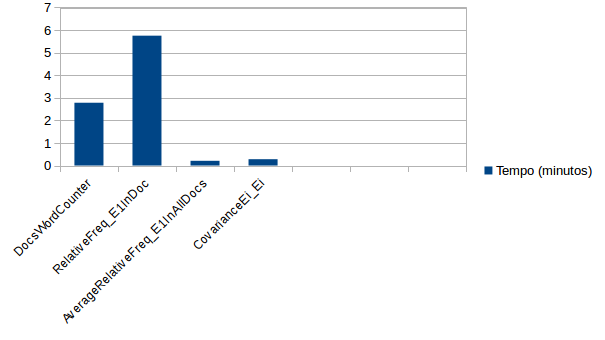
\includegraphics[height=3in]{LaTeX/Chapters/Figures/temposExecucao_Menores.png}
  \caption{Classes com os menores tempo de execução}
  \label{fig:temposExecucao_Menores}
\end{figure}

A classe \textit{ERFile\_Counter} registou um tempo de execução de aproximadamente 2 dias e meio, pois para cada documento é necessário calcular a frequência de cada ER. Ora num \textit{corpus} onde foram extraídas perto de 1 milhão de ERs, seria de esperar que tivessemos tempos de execução muito alargados. 14 segundos foi o tempo estimado para calcular uma covariância entre duas ERs, na classe \textit{CovarianceE1\_E2}. Para que esta pudesse produzir resultados em tempo útil, seria necessário que houvesse uma implementação paralela e distribuída. Para a classe \textit{CorrelationE1\_E2} extimou-se que o cálculo de uma correlação entre duas ERs demorasse cerca de 27 segundos; também neste caso, tornou-se necessária uma implementação paralela e distribuída. É de notar que, os tempos referidos de 14 e 27 segundos resultam de um programa ainda não otimizado. 